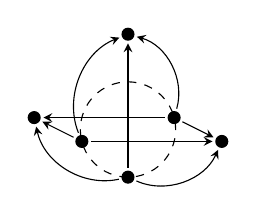
\begin{tikzpicture}
  [junction/.style={fill=KITblack!5},
   point/.style={draw, circle, inner sep=0pt, minimum size=1ex},
   entry/.style={point, fill=black},
   exit/.style={point, fill=white},
   edge/.style={>=stealth, ->, shorten >=1pt, shorten <=1pt},
   original edge/.style={edge, draw=black},
   baseline=(current bounding box.north)]

  \def\JunctionRadius{4ex}
  \pgfmathsetmacro{\Offset}{asin(1ex / \JunctionRadius)}

  \def\Name{J}
  \draw [dashed] circle [radius=\JunctionRadius];
  \node [entry] (\Name-E-en) at (  0 + \Offset:\JunctionRadius) {};
  \node [entry] (\Name-W-en) at (180 + \Offset:\JunctionRadius) {};
  \node [entry] (\Name-S-en) at (270          :\JunctionRadius) {};

  \node [entry, shift={( \JunctionRadius,0)}] (\Name-E-ex) at (  0 - \Offset:\JunctionRadius) {};
  \node [entry, shift={(0, \JunctionRadius)}] (\Name-N-ex) at ( 90          :\JunctionRadius) {};
  \node [entry, shift={(-\JunctionRadius,0)}] (\Name-W-ex) at (180 - \Offset:\JunctionRadius) {};

  \path (\Name-E-en) edge [original edge, ->] (\Name-E-ex);
  \path (\Name-E-en) edge [original edge, ->, bend right=45] (\Name-N-ex);
  \path (\Name-E-en) edge [original edge, ->] (\Name-W-ex);

  \path (\Name-W-en) edge [original edge, ->] (\Name-E-ex);
  \path (\Name-W-en) edge [original edge, ->, bend left=45] (\Name-N-ex);
  \path (\Name-W-en) edge [original edge, ->] (\Name-W-ex);

  \path (\Name-S-en) edge [original edge, ->, bend right=45] (\Name-E-ex);
  \path (\Name-S-en) edge [original edge, ->] (\Name-N-ex);
  \path (\Name-S-en) edge [original edge, ->, bend left=45] (\Name-W-ex);
\end{tikzpicture}
